As we wrote in Section~\ref{subsubsec:design-goals-editor}, we want the user to be able to point at an arbitrary point at the screen, click there and have the program determine which object or place on the floor is being clicked. To be able to do so, the program must first transform the 2D coordinate of the point where the mouse clicked into a 3D coordinate in the scene. This is of course not possible, but it is possible to transform the 2D coordinate into a 3D line. Determining at which cell in a plane (the floor) the user pointed is then a matter of ray-box intersection, which is relatively straightforward to do. It is however not straightforward to determine which object a user has selected. An option is to do ray-box intersection with the ray we have and the bounding boxes of all objects in the scene, but that would be inefficient. Since we may need to do this operation every frame, namely in case the user is hovering the scene and we need to update the position of the ``ghost object'', this is likely too expensive.

A possible solution, that is definitely more efficient, is using Bresenham's algorithm \cite{cohen1994voxel,bresenhamwiki}. This is an algorithm that can be used to find voxels along a line. It is mostly used in 2D to draw a line in a bitmap image for example (see Figure~\ref{fig:bresenham-sketch}), but it can be generalised to 3D. Using this algorithm, one can build a list of all voxels (grid cells) along the viewing ray. Note that because of the way the algorithm works, this list is sorted. That is, the voxels in the list are given from closest away to farthest away (or vice versa of course). To check if there is an object on which the user clicked (and if there is more than one, which one is the closest), one only has to check the voxels in the list, in order. It may be obvious that this is more efficient. There is a downside however: it may happen that an object is selected on which the user did not click, but which is close to the viewing ray. This is because voxels just next to the ray may be selected as well. In practice, this will likely  not be a problem however, as users do mostly not click on the edge of objects to select them. In any case, the program should make it clear which object will be/is selected, so that a user will automatically hover an object more clearly if it is not directly selected.

\begin{figure}[h]
  \centering
  \subfloat[Problem statement: along the line, voxels need to be selected to represent the line in the grid.]{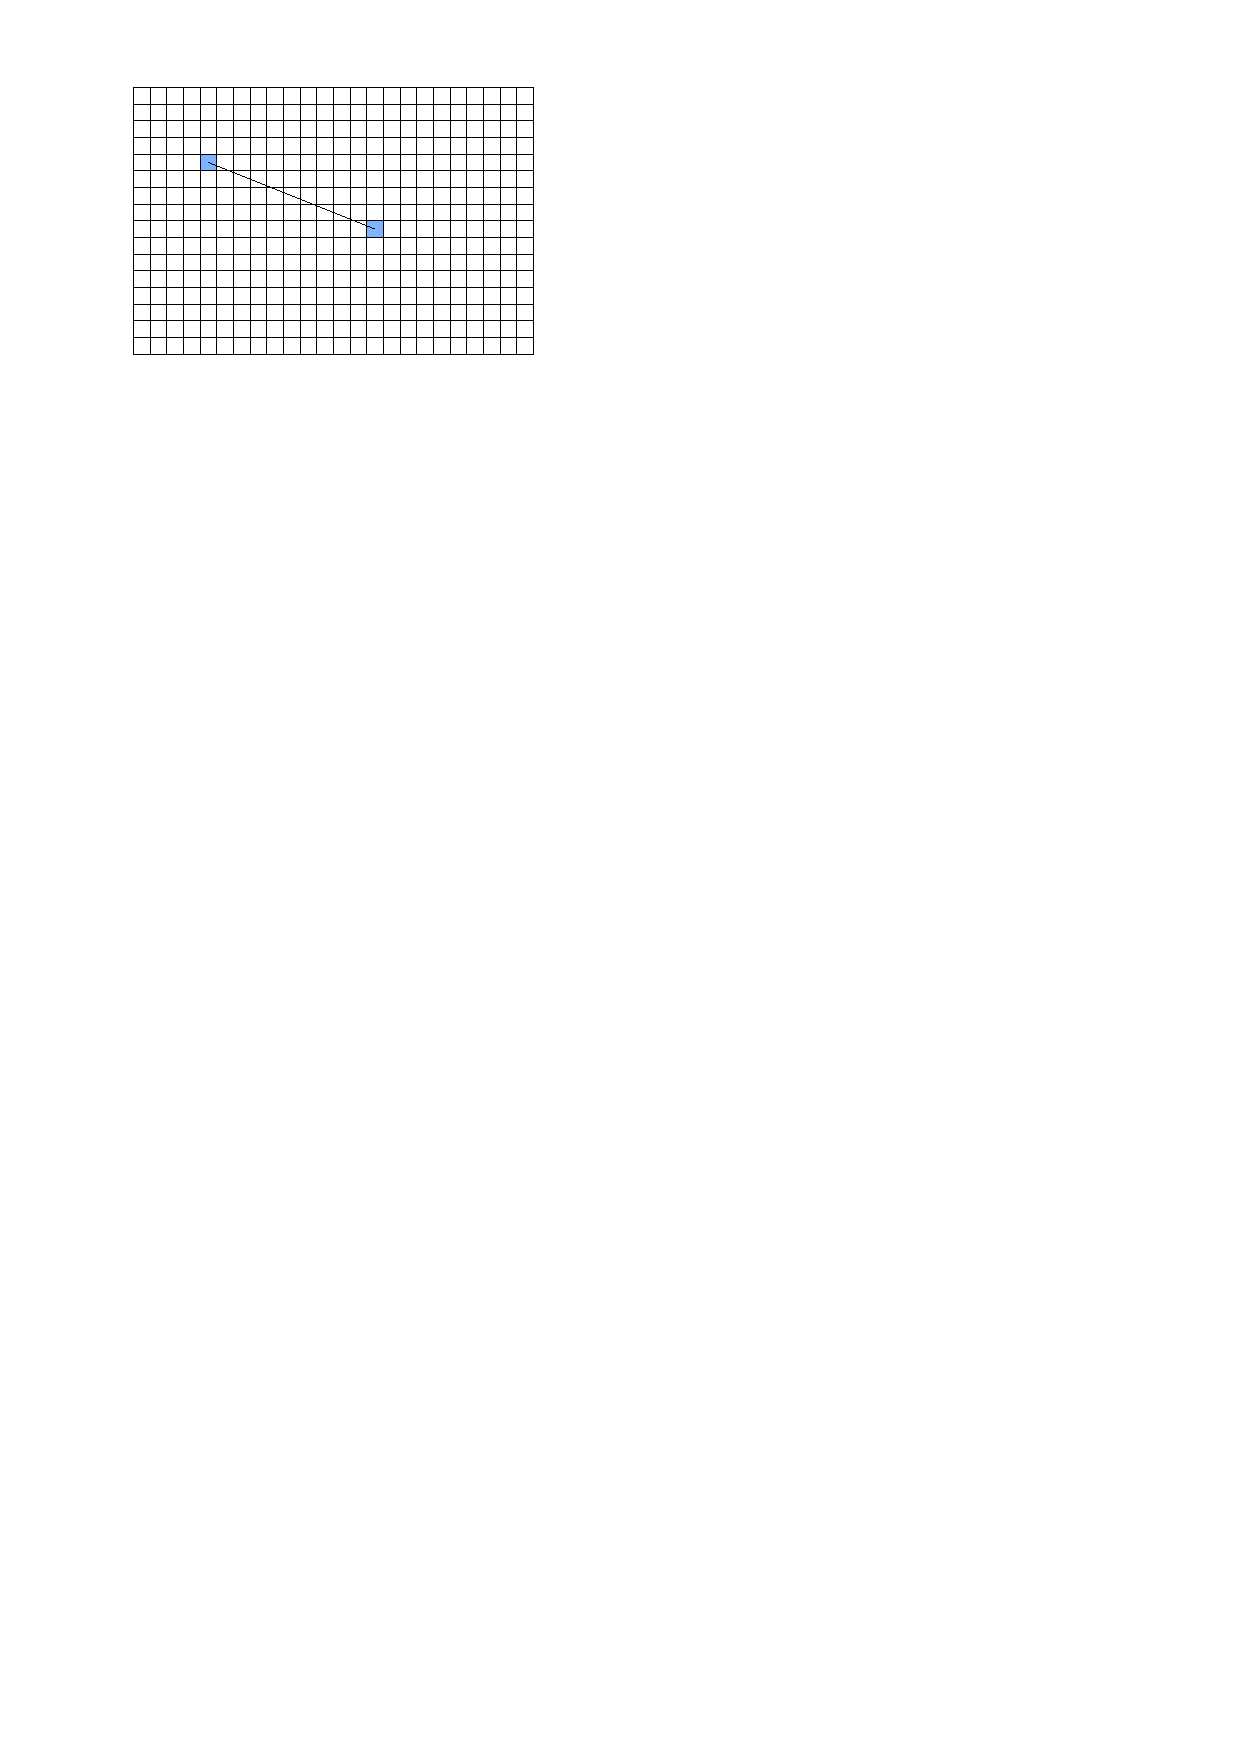
\includegraphics[page=1,width=.3\textwidth]{bresenham}}
  \quad
  \subfloat[Output of ``default version'' of Bresenham's algorithm.]{\includegraphics[page=10,width=.3\textwidth]{bresenham}}
  \quad
  \subfloat[Output of ``extended version'' of Bresenham's algorithm, where more voxels are selected.]{\includegraphics[page=11,width=.3\textwidth]{bresenham}}
  \caption{An illustration of the output of Bresenham's algorithm in 2D.}
  \label{fig:bresenham-sketch}
\end{figure}
